\section{Project Overview}

\begin{frame}
	\begin{figure}[t]
		\centering
		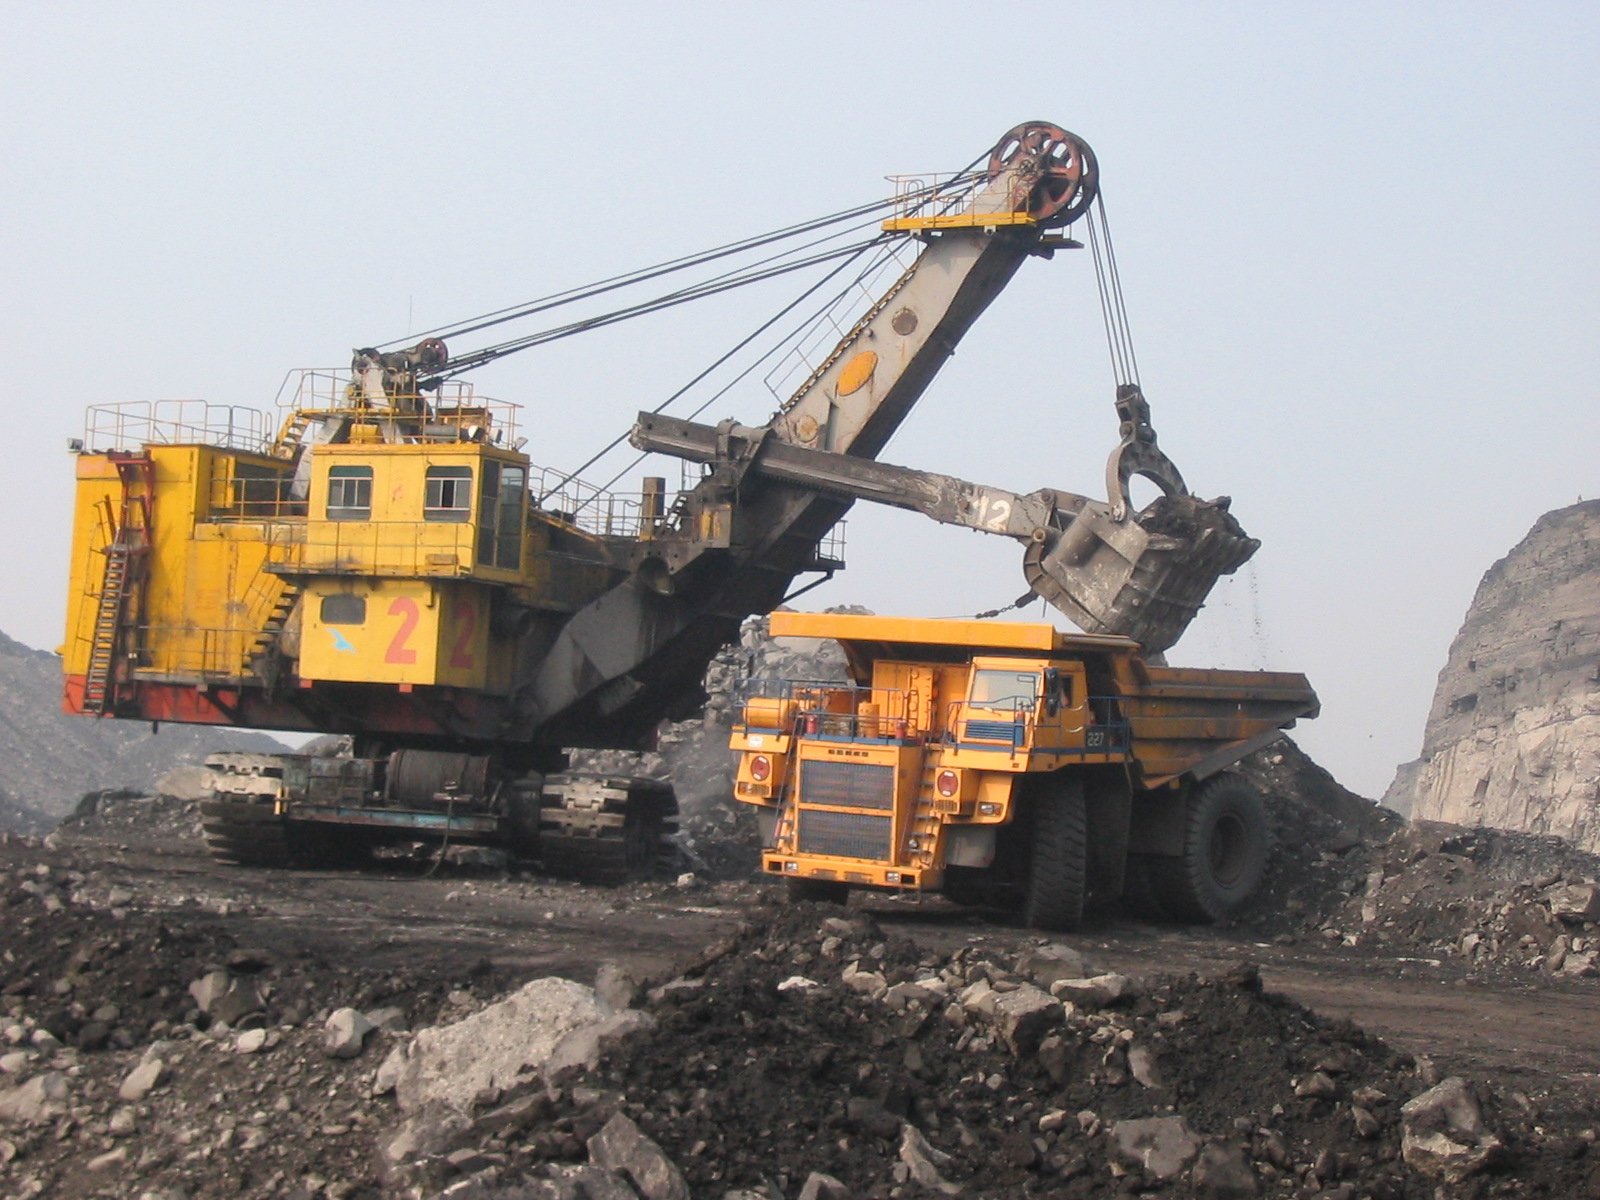
\includegraphics[width=.6\linewidth]{img/Excavator} \\
		\tiny{originally posted to Flickr by FAndrey at http://flickr.com/photos/43301444@N06/4141786255}
	\end{figure}

	\begin{itemize}
		\item{Goal: \textbf{Optimization of model parameters}}
		\item{Models of technical system = Physical properties + Control properties}
	\end{itemize}
\end{frame}


%\begin{frame}
%	\frametitle{Problem Setting}
%	\begin{figure}[bth]
%		\centering
%		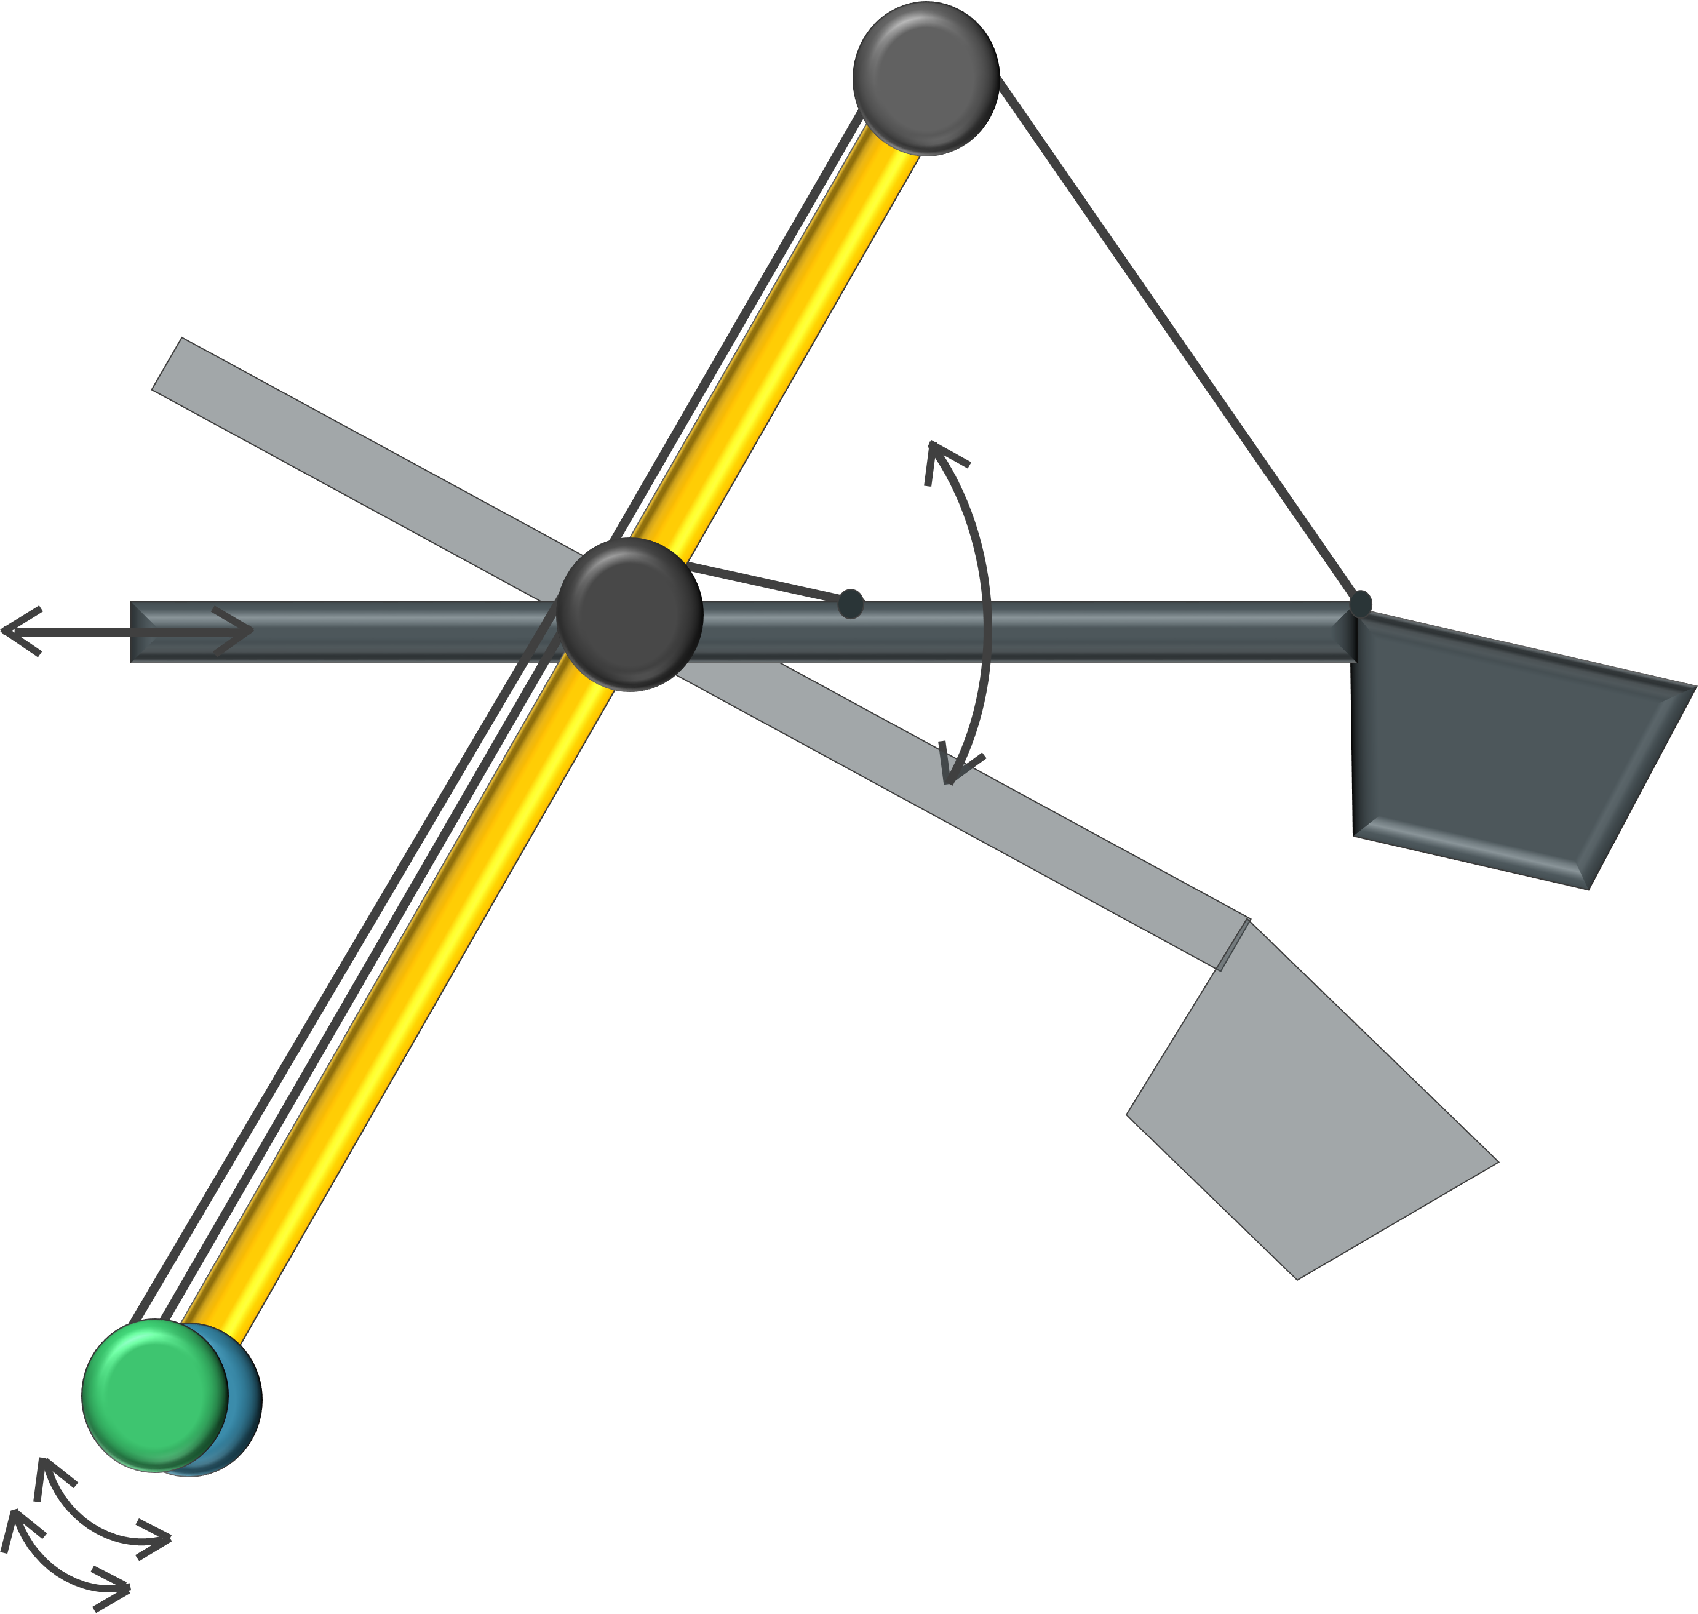
\includegraphics[width=.4\linewidth]{img/Problem_2}
%	\end{figure}
%	\begin{itemize}
%		\item{Arm element fixed to the base}
%		\item{Cannot be moved w.r.t. the base}
%	\end{itemize}
%\end{frame}

%\begin{frame}
%	\frametitle{Problem Setting (include videos)}
%	\begin{figure}[bth]
%		\centering
%		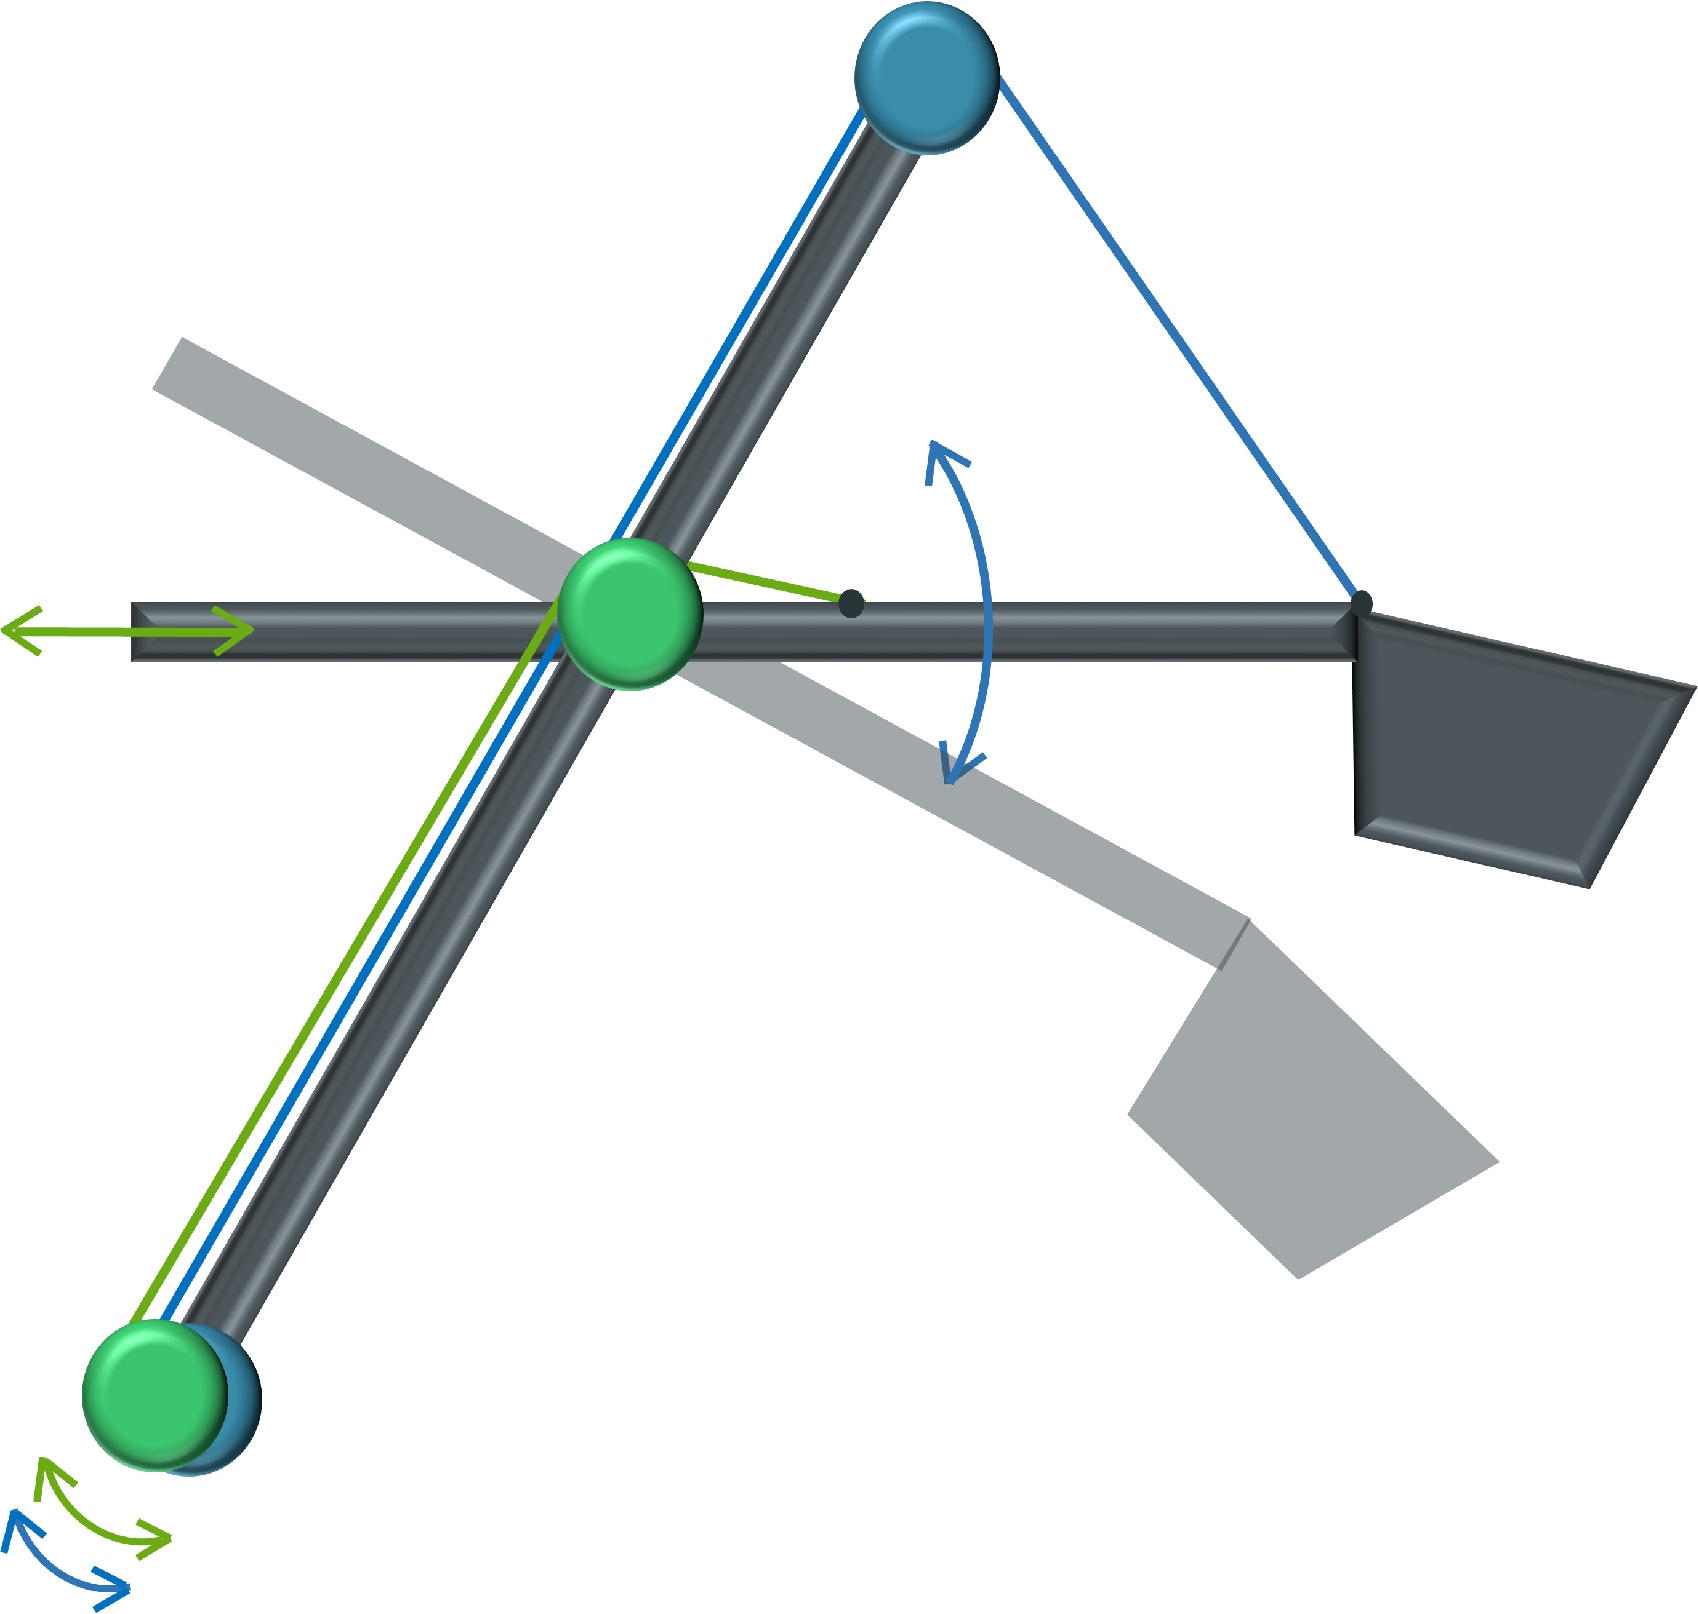
\includegraphics[width=.4\linewidth]{img/Problem_3}
%	\end{figure}
%	\centering
%	\begin{itemize}
%		\item{\makebox[1.5cm][l]{\textcolor[rgb]{0,0.69,0.32}{Green:}} Shovel motion \textbf{back} and \textbf{forth}}
%		\item{\makebox[1.5cm][l]{\textcolor[rgb]{0.18,0.46,0.71}{Blue:}} Shovel motion \textbf{up} and \textbf{down}} \\
%	\end{itemize}
%\end{frame}

\begin{frame}
	\frametitle{Problem Setting}
\centering
\includemedia[
  label      = AA,
  width      = 80mm,
  height     = 50mm,
  activate   = pageopen,
  addresource= videos/ArmMovement.mp4,
  flashvars={flv=videos/ArmMovement.mp4 & autoplay=1 & loop=1}
]{}{player_flv_maxi.swf}
\end{frame}










\begin{frame}
\setbeamertemplate{blocks}[rounded][shadow=false]
    \frametitle{Physical Modeling}
    \vspace{0.3cm}
		\large\textbf{Why?}
		\vspace{1cm}
		\begin{columns}
			\column{.3\textwidth}
				\centering
		    	\begin{block}{}
		    	    \begin{center}
		    	    \vskip 4mm
					{\large Building an accurate model}
					\vskip 3mm
					\hspace*\fill
					\end{center}
				\end{block}
			\column{.1\textwidth}
				\centering
				\Huge{$\Rightarrow$}
			\column{.3\textwidth}
				\centering
				\begin{block}{}
				    \begin{center}
				    \vskip 2mm
					Good description of the effects of control on motion
					%\vskip
					\hspace*\fill
					\end{center}
				\end{block}
		\end{columns}
	\vspace{0.5cm}
\end{frame}
	
	
\begin{frame}
    \frametitle{Physical Modeling}
    \vspace{-0.3cm}
    \large\textbf{How?}
    \vspace{1cm}
	    \begin{columns}
	    \column{0.45\textwidth}
	    \onslide<1->
		To consider:
		\vspace{0.25cm}
		\begin{itemize}
			\item{Friction in cable reels}
			\item{Potential/Kinetic energy}
			\item{etc}
		\end{itemize}
		
		\onslide<2>
		\column{0.1\textwidth}
		    \Huge{$\rightarrow$}
		\column{0.35\textwidth}
		\large\textcolor{red}{Lagrange Formalism}\newline
		\centering{(ODE)}
	\end{columns}
\end{frame}



\begin{frame}
\setbeamertemplate{blocks}[rounded][shadow=false]
	\frametitle{Parameter Identification}
	\onslide<1->
		\large\textbf{What are parameters?}
		\vspace{0.2cm}
		\begin{itemize}
			\item{Friction coefficients}
			\item{Mass}
			\item{Inertia}
		\end{itemize}
	\vspace{0.5cm}
	\onslide<2>
		\large\textbf{Why?}
		\begin{columns}
			\column{.3\textwidth}
				\centering
		    	\begin{block}{}
		    	    \begin{center}
		    	    \vskip 4mm
					 Accurate and realistic parameters
					\vskip 3mm
					\hspace*\fill
					\end{center}
				\end{block}
			\column{.1\textwidth}
				\centering
				\Huge{$\Rightarrow$}
			\column{.3\textwidth}
				\centering
				\begin{block}{}
				    \begin{center}
				    \vskip 2mm
					Better prediction and planning of motion
					%\vskip
					\hspace*\fill
					\end{center}
				\end{block}
		\end{columns}
	\vspace{0.5cm}
\end{frame}
		

\begin{frame}[t]
\frametitle{Visual Examples}

Same parameters except different load weights
\vspace{0.5cm}

\begin{columns}
\begin{column}{0.45\textwidth}


\includemedia[
  label      = AA,
  width      = 50mm,
  height     = 50mm,
  activate   = pageopen,
  addresource= videos/traj_x_095p.mp4,
  flashvars={flv=videos/traj_x_095p.mp4 & autoplay=1 & loop=1}
]{}{player_flv_maxi.swf}
\centering{Light load}
\end{column}


\begin{column}{0.055\textwidth}
	\textbf{vs}
\end{column}


\begin{column}{0.4\textwidth}
\includemedia[
  label      = BB,
  width      = 50mm,
  height     = 50mm,
  activate   = pageopen,
  addresource= videos/traj_x_105p.mp4,
  flashvars={flv=videos/traj_x_105p.mp4 & autoplay=1 & loop =1}
]{}{player_flv_maxi.swf}
\centering{Heavy load}
\end{column}

\end{columns}

\end{frame}



\begin{frame}
    \frametitle{Procedure}
    \onslide<1->
    \begin{columns}[onlytextwidth]
        \begin{column}{0.4\textwidth}
            \begin{block}{\centering{Physical Model}}
         
                    \centering{Lagrange Formalism}
        
            \end{block}
            
            \centering
            $\Downarrow$

            
            \begin{block}{\centering{Parameter Identification}}
            \centering{Discretization + Optimization}
            \end{block}
        \end{column}
        
    \onslide<2>
        
        \begin{column}{0.065\textwidth}
        \textbf{and}
        \end{column}
        
        \begin{column}{0.4\textwidth}
            \begin{exampleblock}{\centering{Blackbox Model}}
                \begin{itemize}
                    \item{Realistic model}
                    \item{Confidential information}
                \end{itemize}
            \end{exampleblock}
            
            \centering
            $\Downarrow$
            
            
            
            
            
            \begin{exampleblock}{\centering{Parameter Identification}}
            \centering{Derivative-free optimization}
            \end{exampleblock}
        \end{column}
    \end{columns}
\end{frame}        
        
        
  

\begin{frame}
	\frametitle{Visualization: Simulink}
	\vspace{-7cm}
	\begin{figure}[t]
	\centering
		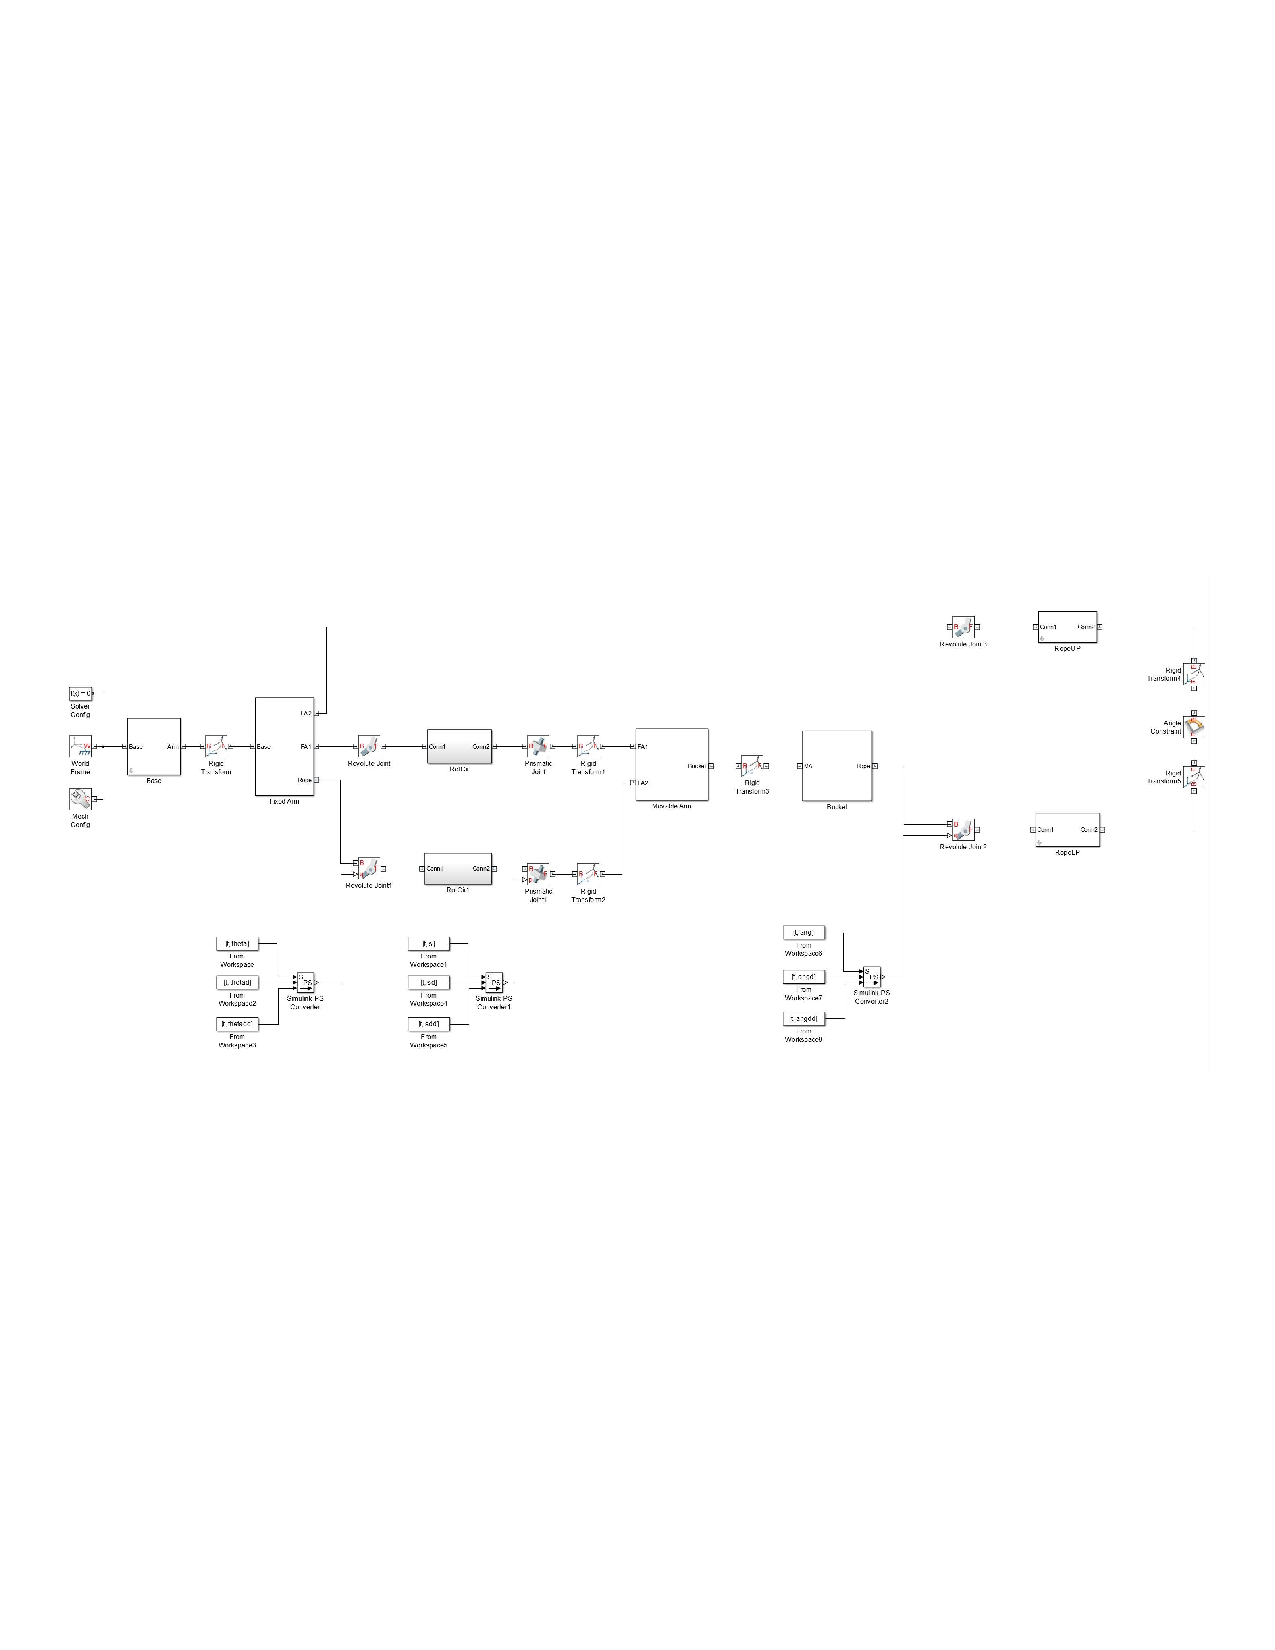
\includegraphics[width=1\linewidth, height=1.5\linewidth]{img/Simulink_Screenshot1}
	\end{figure}
	
	
\end{frame}








   


